\documentclass[fleqn]{article}
\usepackage[spanish,es-noshorthands]{babel}
\usepackage[utf8]{inputenc} 
\usepackage[papersize={6.5in,8.5in},total={5.5in,7.25in},centering]{geometry}
\usepackage{mathexam}
\usepackage{amsmath}
\usepackage{graphicx}
\usepackage{textcomp}
\usepackage{multicol}
\usepackage{tikz,pgf}
\ExamClass{
\includegraphics[height=16pt]{Images/logo-sed.png} Matemáticas $11^{\circ}$}
\ExamName{Funciones}
\ExamHead{
\includegraphics[height=16pt]{Images/logo-colegio.png} IEDAB}
\newcommand{\LineaNombre}{%
\par
\vspace{\baselineskip}
Nombre:\hrulefill \; Curso: \underline{\hspace*{48pt}} \; Fecha: \underline{\hspace*{2.5cm}} \relax
\par}
\let\ds\displaystyle

\begin{document}
\ExamInstrBox{
Respuesta sin justificar mediante procedimiento no será tenida en cuenta en la calificación. Escriba sus respuestas en el espacio indicado. Tiene 45 minutos para contestar esta prueba.}
\LineaNombre
\begin{enumerate}
 \item Exprese la regla en notación de funciones. Por ejemplo, la regla:\\
  ``El cuadrado y luego reste 5'', es expresada en notación funcional como $f(x)=x^{2}-5$
 \begin{enumerate}
  \item El cuadrado de la resta entre $x$ y 4: \dotfill
  \item Reste 3 y luego divida entre la diferencia entre $x$ y 2: \dotfill
  \item La raíz cuadrada de la diferencia entre $x$ y 4: \dotfill
 \end{enumerate}
\item Exprese la función (o regla) en palabras
\begin{enumerate}
 \item $f(x)=\sqrt{x-3}$: \dotfill
 \item $\dfrac{x-4}{x}$: \dotfill
 \item $2x^{2}-3x+1$: \dotfill
\end{enumerate}
\item Complete la tabla para la función dada por $f(x)=x^{2}-3$ y luego grafíquela en el plano

\begin{minipage}{0.5\textwidth}
\begin{tabular}{|c|c|}\hline
$x$ & $f(x)$\\ \hline
--3 & \\ \hline
--2 & \\ \hline
--1 & \\ \hline
0 & \\ \hline
1 & \\ \hline
2 & \\ \hline
3 & \\ \hline
\end{tabular}
\end{minipage}\hfill
\begin{minipage}{0.45\textwidth}
 \begin{tikzpicture}[scale=0.5]
  \draw [dashed,help lines] (-3.5,-3.5) grid (3.5,6.5);
  \draw [thick,<->](-3.5,0)-- (3.55,0)node[right]{$x$};
  \draw [thick,<->](0,-3.5)--(0,6.5)node[right]{$y$};
 \end{tikzpicture}
\end{minipage}
\item Para la función definida a trozos:
\[f(x)=\left\{ \begin{array}{lcl}
              2x-5 & \mbox{si} & x\leq0\\
              x^{2}-2 & \mbox{si} & x>0\\
             \end{array}
\right. \]
Halle:
\begin{enumerate}
\begin{multicols}{2}
 \item $f(-2)=$
 \item $f(-1)=$
 \item $f(0)=$
 \item $f(1)=$
 \item $f(2)=$
 \item $f(\frac{1}{2})=$
\end{multicols}
\end{enumerate}
%\item Para la función $f(x)=3x^{2}-2x+4$ halle:
%\begin{enumerate}
% \item $f(a)=$\vspace{10pt}
% \item $f(2x)=$\vspace{10pt}
% \item $2f(x)=$\vspace{10pt}
% \item $f(x+1)=$\vspace{10pt}
% \item $f(x)+f(1)=$\vspace{10pt}
% \item $f(a+h)=$
%\end{enumerate}
\item Dada las funciones del gráfico (página siguiente), encuentre:

\begin{minipage}{.45\textwidth}
\begin{tikzpicture}[scale=.75,domain=-2:2.1,smooth]
\draw[dashed,help lines] (-2,-2)grid(2,4);
\draw[<->](-2.2,0)--(2.2,0)node[below]{$x$};
\draw[<->](0,-2.2)--(0,4.2)node[right]{$y$};
\draw plot (\x,4*\x*\x-\x*\x*\x*\x)node[right]at(1.5,3.5){$f$};
\draw plot (\x,-\x*\x+3) node[right] at (0,3.15){$g$};
\end{tikzpicture}
\end{minipage}
\begin{minipage}{.5\textwidth}
\begin{enumerate}
%\begin{multicols}{2}
\item $f(0)=$\noanswer
\item $g(0)=$\noanswer
\item $f(-2)=$\noanswer
\item $g(-1)=$\noanswer
\item $f(-1)=$\noanswer
\item $f(1)=$\noanswer
\item $g(1)=$\noanswer
%\end{multicols}
\end{enumerate}
\end{minipage}
\item La gráfica muestra la temperatura de un enfermo entre las
0h y 22h.
\begin{center}
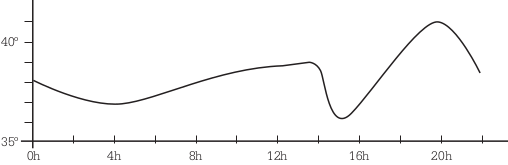
\includegraphics[scale=.5]{Images/PantallazoFunc.png} 
\end{center}
\begin{enumerate}
\item ¿Hubo algún descenso de temperatura durante la madrugada?¿Entre qué horas?\noanswer
\item ¿Cuál fue la temperatura a las 14h?\noanswer
\item ¿A qué hora la temperatura fue de 37\textcelsius? \noanswer
\item Halla e interpreta la imagen de 4 y la anti-imagen\footnote{La anti-imagen es el número del cual se es imagen: Por ejemplo, si $f(3)=5$, entonces la anti-imagen de 5 es 3 y se escribe $f^{-1}(5)=3$} anti-imágenes de 38\textcelsius.\noanswer
\item En un momento dado el enfermo sufrió un brusco descenso de la temperatura. ¿Cuándo?\noanswer
\item ¿Tuvo el enfermo algún momento de peligro?\noanswer
\item Estudia e interpreta el crecimiento de la función y sus
máximos y mínimos relativos.\noanswer
\end{enumerate}
%\item En una empresa el costo de producir un computador es $c$. Si se venden $y$ computadores con un precio de $v$ cada uno, entonces la expresión correcta para la ganancia $g$ es:
%\begin{enumerate}
%\item $g=y(v+c)$
%\item $g=vy-c$
%\item $g=c-vy$
%\item $g=y(v-c)$
%\end{enumerate}


%\section*{Probabilidad}
%\item Si se lanzan un par de dados y $P(6)$ indica la probabilidad de que la suma de los números superiores del dado sea 6, entonces halle:
%\begin{enumerate}
%\begin{multicols}{2}
%\item $P(5)=$\noanswer
%\item $P(4)=$ \noanswer
%\item $P(3)=$\noanswer
%\item $P(2)=$\noanswer
%\end{multicols}
%\end{enumerate}
%\item Se lanzan tres monedas simultáneamente, encuentre:
%\begin{enumerate}
%\item El espacio muestral $S$ \noanswer%$S=\{ccc,ccs,csc,scc,css,scs,ssc,sss\}$
%\item La probabilidad de obtener dos caras:\noanswer
%\item Obtener solamente una cara:\noanswer
%\item La probabilidad de obtener tres caras:\noanswer
%\end{enumerate}
 \end{enumerate}
\end{document}
